\section{Mission1 Development Results}
\label{sec:native}
\subsection{Evidence and expenditure under common caps}
The initial pilot serializes four policies at four caps before assessment. Every
arm emits one packet per active hour and respects its encoded cap. Decoding checks
raw values and timestamps exactly and summaries against their true source buckets.
All 11 annotated evaluation anomalies have eligible original observations, so a
retention failure remains a miss under a shared denominator.

At 1,024 bytes per active hour, adaptive capture preserves PCA evidence for 11/11
events using 6.30 MiB, compared with 5/11 and 25.04 MiB for uniform sampling.
Pre-event context averages 64.3\% versus 22.9\%. The unconstrained format cost,
calculated from source records and hourly headers rather than serialized as a
fifth policy, is 112.34 MiB. Threshold-only capture uses 0.81 MiB and preserves
10/11 events, exposing a cost/evidence tradeoff rather than a universal winner.

\subsection{Seeded controls and component removals}
Reservoir sampling uses Algorithm R; randomized-phase sampling shifts the equal-
time targets and skips targets crossed by native gaps. Both use bounded epoch
state and retain each observation at most once. Seeds 0--9, all four caps, and the
two policies give 80 arms. Epoch-specific seeds prevent skipped epochs from shifting
later random sequences; budgets share random numbers without guaranteeing nested
reservoirs. All comparisons reuse the original frozen receiver parameters.

At 1,024 bytes, reservoir retains a mean 5.1 PCA events (observed seed range 4--7)
using 25.15 MiB, and randomized phase 5.4 (4--8) using 24.96 MiB. Their mean context
coverage is 23.8\% and 21.8\%. Figure~\ref{fig:seeded} shows the four-cap tradeoff.
These ranges describe variation on the same 11 events. Uniform's nonmonotonic
coverage across caps is possible because changing strata changes phase.

\begin{figure}[htbp]
\centering
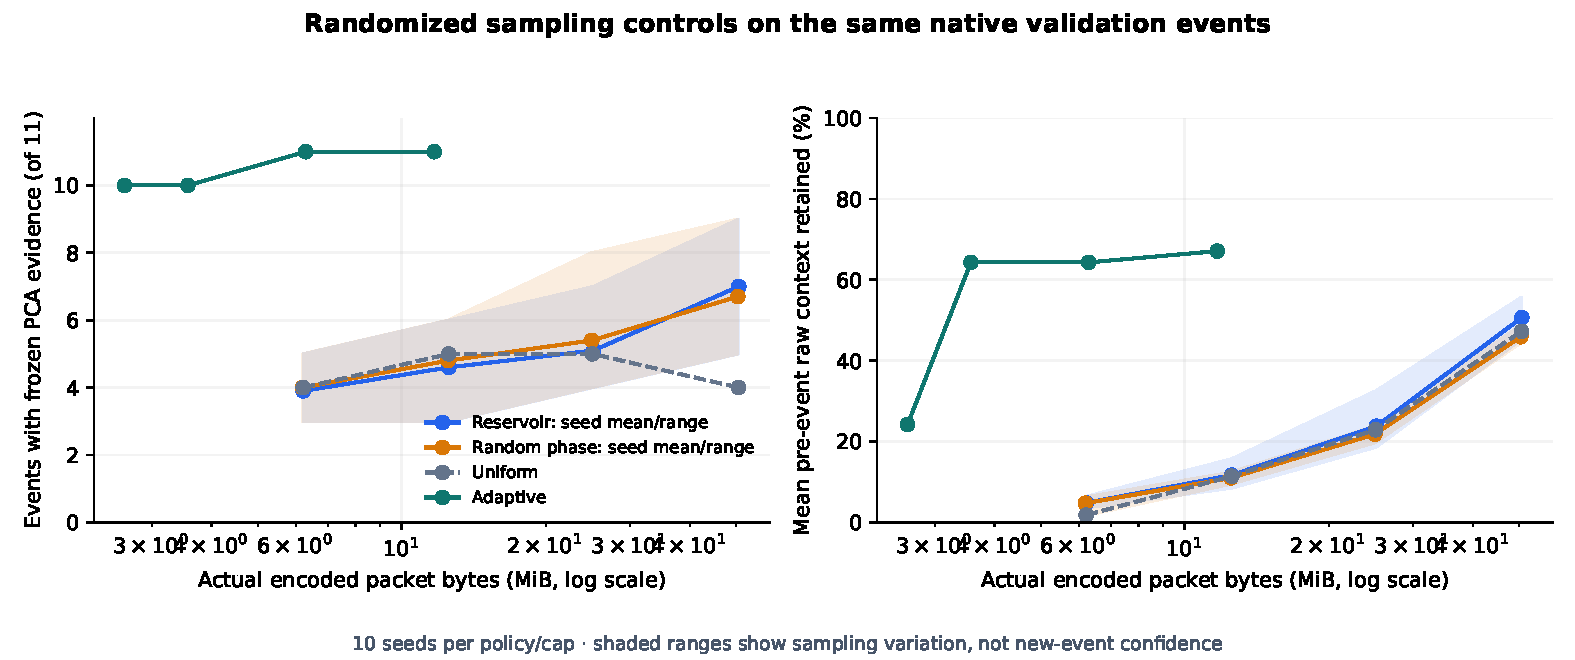
\includegraphics[width=\linewidth]{generated/randomized_tradeoff.pdf}
\caption{Mission1 evidence and context against actual encoded bytes. Shading is
the observed seed range, not a confidence interval for new faults. Shared caps
allow different actual expenditure.}
\label{fig:seeded}
\end{figure}

Sixteen paired ablation arms remove one component at a time. Full arms reproduce
the original adaptive packet bytes exactly. At 1,024 bytes, removing pre-trigger
capture preserves 11/11 PCA events while reducing pre-context from 64.3\% to 1.8\%.
Removing background reservation loses PCA evidence for event \texttt{id\_138} and
reduces cost from 6.30 to 0.90 MiB. At 256 bytes, releasing the background quota
instead increases pre-context from 24.2\% to 41.5\%. Thus reservation has a
budget-dependent opportunity cost. Removing post-trigger capture leaves PCA event
counts and pre-context unchanged at every cap; diagnostic post-event usefulness
has not been established. These removals do not estimate component interactions.

\subsection{Receiver mismatch and the temporal limitation}
\label{sec:mismatch}
The expanded benchmark crosses four capture conditions with threshold, adaptive,
and coverage recording, alongside uniform and seeded controls: 132 arms total.
At 1,024 bytes, adaptive and coverage retain rank-three PCA evidence for 11/11
events at approximately 6.30 MiB. Coverage raises pre-context from 64.3\% to
66.3\% but reduces post-context from 40.2\% to 36.9\%. At PCA ranks four and
five, coverage retains 11/11 and ordinary adaptive capture 10/11. With the trigger
disabled, their rank-three counts are 6/11 and 4/11 at 6.22 MiB. These are
correlated receiver sensitivities, not broad detector-independent guarantees.

The AR(1) receiver is calibrated on 8,712,785 eligible training pairs. Full-archive
input supplies evidence for all 11 events. Seven declared policies at four caps
give 28 temporal assessments. At 1,024 bytes, adaptive context preserves temporal
evidence for 10/11 events, uniform for 2/11, and threshold-only for 1/11. Disabled-
trigger singleton background retains 0/11 temporal events despite 4/11 PCA events.
Isolated retained values therefore cannot be treated as usable forecast transitions.

The pair control is introduced after observing that validation failure and assessed
in eight exploratory arms. Under enabled first-difference capture, it matches
adaptive's 10/11 temporal events at the 1,024-byte cap. With the trigger disabled,
it retains 2/11 temporal and 4/11 PCA events at 6.22 MiB. It partially addresses
the measured input failure without establishing optimal allocation or general
protection of unfamiliar faults. Table~\ref{tab:temporal} reports cost and input
availability alongside event counts; Figure~\ref{fig:requirements} contrasts this
development result with the frozen follow-up.

\begin{table}[htbp]
\centering\small
% Generated temporal receiver and adjacent-pair comparison.
\begin{tabular}{lrrrr}
\toprule
Capture / policy & MiB & PCA events & AR(1) events & Retained pairs \\
\midrule
Uniform & 25.04 & 5/11 & 2/11 & 2957 \\
Diff. / threshold & 0.81 & 10/11 & 1/11 & 11 \\
Diff. / adaptive & 6.30 & 11/11 & 10/11 & 1057 \\
Diff. / coverage & 6.30 & 11/11 & 10/11 & 4886 \\
Level / adaptive & 6.67 & 11/11 & 10/11 & 7281 \\
Pca / adaptive & 8.86 & 11/11 & 10/11 & 69167 \\
Disabled / adaptive & 6.22 & 4/11 & 0/11 & 0 \\
Diff. / burst & 6.30 & 11/11 & 10/11 & 79668 \\
Disabled / burst & 6.22 & 4/11 & 2/11 & 78877 \\
\bottomrule
\end{tabular}

\caption{Mission1 at 1,024 bytes per hour. Pairs require consecutive original
observations within the gap limit; input counts include periods excluded from
fault scoring. Burst rows are exploratory. Exact bytes and complete cap results
are in the reports.}
\label{tab:temporal}
\end{table}
